\documentclass[../main.tex]{subfiles} 
\begin{document}

\chapter{TEORETISK GRUNNLAG}

Denne seksjonen beskriver de viktigste begrepene, konseptene og teknologiene som er brukt som grunnlag for utvikling, gjøre vurderinger samt å beskrive metode og resultat i prosjektet. Noen av beskrivelsene vil også inneholde bilder eller kodeeksempler.

\section{Arkitekturer, teknologier og konsepter}

Denne delen tar for seg de forskjellige teknologier, arkitekturmodeller og konsepter som er benyttet som designgrunnlag for prosjektet og er ellers omtalt i rapporten. Inndelingen av seksjoner er satt opp hierarkisk (dvs. at f.eks teknologier som tilhører en annen teknologi befinner seg i en underseksjon), og lineært oppbyggende. Det sistnevnte innebærer at tidligere delen av seksjonen gir grunnlag for å enklere forstå senere deler.

\subsection{Systemintegrasjon}

\subsubsection{Definisjon}
Systemintegrasjon er å få to eller flere systemer til å samhandle. Det har også blitt definert som "å bringe subsystemer sammen i et system, og forsikre at subsystemene arbeider sammen i systemet" \endnote{ \url{https://en.wikipedia.org/wiki/System_integration} - 22.05.2013}. \newline
\newline
Systemintegrasjon kan gjennomføres ved å få de aktuelle systemene til å snakke med hverandre, det ene snakker til det andre(som en slags monolog). I situasjoner hvor det er mer enn to systemer kan det være en kombinasjon av de to løsningene. Det kan også forekomme at mellom to(eller flere) systemer blir det implementert et tredje program som har som oppgave å koordinere de andre.\newline
\newline
I systemintegrasjon snakker man ofte om cohesion, eller grad av avhengigghet. Dette refererer til hvor mye de forskjellige subsystemene er avhengige av hverandre. Man ønsker å ha så lav cohesion som mulig samtidig som at systemet må kunne utføre de oppgavene som kreves av det. \endnote{\url{http://en.wikipedia.org/wiki/Cohesion_(computer_science)} - 25.05.2013}\newline
\newline
I systemintegrasjon finnes det en del forskjellige måter for programmer å samhandle. Her følger en kort beskrivelse av de vanligste metodene:

\subsubsection{Data Scraping}
Data-scraping er en teknikk som involverer bruken av software-program til å hente ut spesifikk og meningsfull data fra et annet datasett formatert for å presentere menneskeleselig data. \endnote{\url{http://en.wikipedia.org/wiki/Data_scraping} - 28.05.2013} \endnote{\url{http://onlinejournalismblog.com/2010/07/07/an-introduction-to-data-scraping-with-scraperwiki/} - 28.05.2013}\newline Begrepet menneskeleselig beskriver informasjon formatert på en måte beregnet for å kunne vises til og forstås av en sluttbruker. Dette innebærer ofte at den relevante informasjonen man søker er omsluttet av irrelevant eller redundant data, eller befinner seg uforutsigbart plassert i datasettet. Fordi datastrukturen dermed ikke egner seg for videreføring av data mellom programmer, skiller data-scraping fra syntaktisk \endnote{\url{http://snl.no/syntaktisk} - 28.05.2013} data-analyse eller parsing som benytter seg av etablerte formateringsregler. Man kan si at data-scraping går ut på å gjøre ellers utilgjengelig data tilgjengelig for forståelse av programmer, eller å sette ustrukturert data i system.\newline
\newline
Web-scraping (se begreper) er en mer spesifikk teknikk innen data-scraping for å lokalisere og hente ut data fra nettsider som inneholder ustrukturert data. En nettside svarer typisk med data formatert som HTML, og selve scraping-delen vil da bestå i å filtrere vekk unødvendig data, og plukke ut og sortere relevant data programmatisk. 

\subsubsection{API}

Et API (Application Programming Interface) er et grensesnitt som gir eksterne brukere og applikasjoner tilgang til en annen applikasjons eller systems tjenester, funksjoner og data. \endnote{\url{https://en.wikipedia.org/wiki/Application_programming_interface} - 27.05.2013}Ved bruk av API kan man bygge store modulære systemer. Dette vil også si at om man vil endre måten programmet fungerer på, så kan man det uten at det påvirker andre program som avhenger av det så lenge man beholder den samme API’en. \endnote{\url{http://money.howstuffworks.com/business-communications/how-to-leverage-an-api-for-conferencing1.htm} - 27.05.2013}

\subsubsection{Fil-dump baserte systemer}

Eldre datasystemer hadde ofte ikke tilgang på store mengder minne. Variabler og mellomlagring av data måtte derfor skrives til disk. Dette gjorde at om man ville hente inn data fra et fil-dump basert program, måtte man lese fra disse filene. Den største ulempen med denne metoden er at disk IO er veldig tregt i forhold til IO fra minne, så disse operasjonene var generelt ganske trege. Et annet problem var samtidighet mellom flere kilder når de vil lese og/eller skrive til/fra den samme kilden. Om et program skriver til en fil samtidig som et annet leser fra den, kan det oppstå feil. Dette er riktignok håndtert automatisk i nyere operativsystemer, men det kan fortsatt oppstå feil hvor et program ikke gir fra seg rettighetene til å lese/skrive til en fil.\newline
Selv om dette er en lite brukt måte å utvikle systemer på idag, finnes det fremdeles i bruk i <------------------------------------

\subsection{Robots.txt}

Dette er en protokoll som brukes av nettsider til å fortelle nettjenester om de få lov til å innhente data automatisk. De vanligste tjenestene som bruker denne sjekken er søkemotorer(google, yahoo etc.), men den er aktuell for alt og alle som vil innhente data fra en nettside eller tjeneste.\newline
Protokollen kan forby tilgang til deler av sin egen mappestruktur, eller for å blokkere spesifikke tjenester(ofte blokkere søkemotorer). Det er viktig å merke seg at denne protokollen ikke aktivt blokkerer noe som helst, men fungerer som internettets trafikkskilt. Det vil si at protokollen ikke hindrer deg i å gjøre noe, men den viser om det er lov eller ikke.

\subsection{Model View Controller}
\begin{figure}[H]
  \centering
    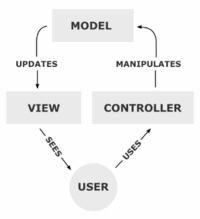
\includegraphics[width=0.3\textwidth]{mvc.png}
   \caption{Model View Controller-modellen}
\end{figure}

Model View Controller (MVC) er en arkitektur for programvare som begrenser hvilke deler av programmet brukeren interagerer med. "Model"-delen er kjernen i applikasjonen og består av dataen til applikasjonen (databasen), applikasjonslogikk, metoder og funksjoner. "View"-delen består av den informasjonen fra modell-laget som er tiltenkt brukeren som for eksempel tekst, bilde, lyd osv. "Controller" delen består av håndtering av brukerens input for å styre de to andre lagene. \endnote{Ed Lecky-Thompson, Heow Eide-Goodman, Steven D. Nowicki og Alec Cove, Professional PHP5 (Wiley Publishing, Inc , 2005)}

\subsection{Web Services}

En web service, eller nett-tjeneste, er en mekanisme som muligjør kommunikasjon eller tilbyr tilgang til funksjoner\endnote{Frank Trethan Johnsen, Web services and service discovery(Kjeller : Norwegian Defence Research Establishment, 2008), 9} over et nettverk \endnote{Mike Jasnowski, Java, XML, and Web Services Bible(Hungry Minds Inc, 2002)}. Slike nett-tjenester bruker typisk HTTP/HTTPS over internett, og er dermed en form for distribuert system hvis tilhørende komponenter tilgjengelig for en bred rekke av enheter\endnote{Java Web Services - Up and running, Forfatter: Martin Kalin, Forlag: O’Reilly Media, Inc, År 2009}. Det finnes flere typer nettjenester og kan deles grovt i to grupper, SOAP- og REST-baserte nett-tjenester. \endnote{Kim Topley, Java Web Services in a Nutshell (O Reilly, 2003)} \endnote{Java Web Services - Up and running, Forfatter: Martin Kalin, Forlag: O’Reilly Media, Inc, År 2009}

\subsubsection{REST}

REST (Representational State Transfer) er en ikke-protokoll-spesifikk dataoverførings-arkitektur bestående av klienter og servere. Denne arkitekturen beskriver en del begrensinger som når benyttet i et distribuert system fører til nyttige egenskaper som loose coupling og horisontal skalerbarhet. \endnote{RESTful Java with JAX-RS, Forfatter: Bill Burke. O’Reilly Media, Inc, År 2003} En typisk REST transaksjon kan beskrives på følgende måte; en klient sender en forespørsel til en server, som bearbeider forespørselen og sender tilbake data. Måten dette foregår på, metodene og standardene som benyttes er hva begrensningene definerer. Nettjenester som er designet i tråd med REST’s arkitektur-prinsipper kalles "RESTful services".\newline
\newline
Grunnleggende arkitekturprinsipper i REST:

\begin{itemize}
\item \textbf{Addressability} \newline
Ethvert objekt or enhver ressurs i et system skal være tilgjengelig gjennom en unik identifikator. (URI)
\item \textbf{The Uniform, Constrained Interface} \newline
Kun operasjoner som er definert innenfor protokollen tjenesten bruker er tillatt. Det skal med andre ord ikke opprettes egne funksjoner for handlinger i URI’en. I eksempelvis HTTP begrenser man seg til metodene som GET, PUT, DELETE, POST, etc...
Formålet med dette er b.la å gjøre tjenesten lettere forståelig ved å bygge på eksisterende terminologi og funksjonalitet.
\item \textbf{Representation-Oriented} \newline
En ressurs skal representeres i en dataoverføring tilbudt av en nett-tjeneste. En hent-operasjon skal gi tilbake en representasjon av ressursen, og en endrings-operasjon skal sende en representasjon av ressursen som skal endres.
\item \textbf{Stateless communication} \newline
Det skal ikke lagres sesjonsdata på serveren. Serveren skal kun håndtere tilstanden til resursser som er tilbudt gjennom nett-tjenester.
\item \textbf{HATEOAS (Hypermedia As The Engine of Application Sate)} \newline
Dataformatet skal styre tilstandsendringe i applikasjonen. Hvis det er nødvendig å begrense tilgang eller aksessere tjenesten på en spesiell måte, skal dette håndteres av hypermedia (f.eks en nettside)
\end{itemize}
REST bruker API-ressurslinker (URI) for å aksessere resursser, eksempel på dette kan være: URL for å hente en kunde med ID 32133:

\begin{lstlisting}[language=HTML, frame=single]
http://customers.myintranet.com/customers/32133
\end{lstlisting}

\subsubsection{URI-design}

En URI tjener som en identifikator til endepunkt i et system som tilbyr web-services. Defineringen og utformingen av disse URI’ene har dermed mye å si for de som vil aksessere disse endepunktene, enten om de er programvareutviklere eller vanlige brukere. I et RESTful system vil en URI sørge for addressability-prinsippet, og en RESTful URI burde derfor følge arkitekturprinsippene så langt det er anvendbart. \endnote{Java Web Services - Up and running, Forfatter: Martin Kalin, Forlag: O’Reilly Media, Inc, År 2009}

\subsubsection{Dataformater}

Denne delen beskriver forskjellige dataformat som har blitt benyttet i prosjektet og er relevant ellers for denne rapporten.

\paragraph{JSON}
JSON (JavaScript Object Notation) er et lettvekts dataformidlingsformat basert på delsyntaks fra JavaScript. Enkelheten i JSON ligger i at det er lettlest og lettskrevet av mennesker, noe som gjør det å arbeide med JSON til en relativt enkel oppgave sammenlignet med formater med lignende funksjonsområder. (bla. XML).\newline
I hovedsak er JSON basert på nøkkel/verdi-par og lister som har en nøkkelverdi som identifikasjon. Som nøkkelverdier bruker JSON strenger som demonstrert i figuren nedenfor:

\begin{lstlisting}[language=HTML, frame=single, caption={(JSON-formatert data)}]

{
    day: "Man",
    date: "7 jan",
    lectures:  [
        {
             lectureStart: "08:15",
             lectureEnd: "10:00",
             type: "Foreles",
             classId: "AU1, DA1, AU-y1, DA-y1",
             room: "Borgundfjorden",
             teachers: "Blom Martin",
             comment: null,
             courses:  [
                 {
                      courseName: "Fysikk og kjemi",
                      courseID: null
                 }
             ]
    ]
}

\end{lstlisting}

Verdiene som er knyttet til en nøkkel kan være av følgende typer:
\begin{itemize}
\item Strenger
\item Boolske verdier (true/false)
\item Matriser
\item Objekter (en liste med nøkkel/verdi-par)
\item Null-verdier
\end{itemize}

JSON blir ofte brukt til serialisering av data som skal sendes mellom server- og klientapplikasjoner. JSON er plattform-uavhengig. \endnote{CouchDB - The Definitive Guide, Forfatter: J.Chris Anderson, Jan Lehnardt, Noah Slater, Forlag: O’Reilly Media, Inc, År: 2010)} \endnote{\url{http://www.json.org/} - 6.05.2013} \endnote{\url{http://en.wikipedia.org/wiki/Json} - 6.05.2013}

\paragraph{XML}

XML er et dataformat som er ment å kunne leses både av mennesker og av maskiner. Mange nettjenester bruker formatet til å representere og strukturere svardata for deres API’er. \endnote{\url{http://en.wikipedia.org/wiki/XML} 30.05.2013} \endnote{\url{http://www.w3schools.com/xml/xml_whatis.asp} - 30.05.2013}

\subsection{AJAX}

AJAX (Asynchronous JavaScript and XML) er en gruppe teknologier brukt til å lage asynkrone klientside-funksjoner i webapplikasjoner. Dette vil si at med AJAX kan nettsider laste inn og sende data etter innlastingen av selve nettsiden, dette kan forenkle flyten i webgrensesnittet ved at brukeren kan gjøre endringer uten å måtte laste hele siden på nytt. \endnote{\url{http://en.wikipedia.org/wiki/Ajax_(programming)} - 15.05.2013} \endnote{Steve Souders, Even Faster Web Sites(O`Reilly Media Inc, 2009), 5}

\section{Programmering}

Denne delen tar for seg de forskjellige programspråkene og teknikkene som er benyttet i prosjektet.

\subsection{Java}

Java er et objektorientert programmeringsspråk originalt utgitt av Sun Microsystems i 1995. Det er et språk hvor alt behandles som objekter, og hvor objektene kan samhandle for å utføre oppgaver. Språket er mest kjent for sin evne til å fungere på alle plattformer uten å måtte rekompilere koden. Dette prinsippet kalles Write Once, Run Anywhere(WORA), og det var Java som var først ute med denne løsningen. \endnote{\url{http://www.computerweekly.com/feature/Write-once-run-anywhere} - 20.05.13}
Språket er utviklet med fem hovedmål \endnote{\url{http://www.oracle.com/technetwork/java/intro-141325.html} - 20.05.13}:
\begin{itemize}
\item Det skal være enkelt, objektsorientert og kjent(ligne på andre språk)
\item Det skal være robust og sikkert
\item Det skal være plattform uavhengig
\item Det skal ha høy ytelse
\item Det skal tolkes, genereres tråder og være dynamisk i sanntid
\end{itemize}
Java brukes i dag til et bredt spekter av formål og til mange forskjellige typer enheter. Dette innebærer bruk som webtjenere(nettsider etc.), enkeltstående applikasjoner(normale programmer) og innebygde systemer(vaskemaskiner, kaffemaskiner etc.). 

\subsubsection{Teknisk}

Java applikasjoner, eller programmer kjører på en virtuell maskin som heter Java Virtual Machine(JVM). Dette betyr at applikasjonen kjører på en virtuell datamaskin. Dette vil si at uansett hvilken fysisk maskin applikasjonen kjører på, vil alltid maskinen se lik ut for applikasjonen. Om det gjøres systemkall til operativsystemet, oversetter den virtuelle maskinen dette for applikasjonen. \endnote{\url{http://www.java.com/en/about/} - 28.05.2013}

\subsection{Regulære uttrykk og Java}

Et regulært uttrykk (ofte forkortet "regex") er en streng med karakterer som utgjør et mønster, som igjen beskriver eller matcher en eller flere strenger. \endnote{Regular Expression’s Cookbook, Forfatter: Jan Goyvaerts, Steven Levithan, Forlag: O’Reilly Media, Inc, År: 2009)} Et slikt uttrykk brukes for å søke etter grupper av sammenhengende tekst, som da kan behandles på ønsket måte. Med unntak av spesielle karakterer, vil et regulært uttrykk beskrive en streng karakter for karakter, hvor f.eks det regulære uttrykket "regex" vil matche det første tilfellet av strengen "regex" i en annen tekststreng. De spesielle karakterene definert i syntaksen oversettes til en spesiell handling eller kan alene definere flere karakterer i en tekststreng. \newline
Syntaksen i et regulært uttrykk varierer med implementasjonen da programmeringspråk eller programmer som har støtte for regulære uttrykk benytter seg av forskjellige prosesserings-motorer, eller har sin helt egen variant av konseptet. Til tross for dette, er likevel syntaksen svært lik hvis ikke helt identisk i de fleste tilfeller hvor de regulære uttrykkene baserer seg på Perl. Eksempelvis i Java er det noen slike forskjeller, som siden versjon 4 har støtte for regulære uttrykk vært tilbudt gjennom \textbf{java.util.regex} pakken, og baserer seg på Perl’s implementasjon. Et regulært uttrykk i Perl kan være strengen "\\w", en spesiell karakter, som vil beskrive enhver streng med én bokstav, bindende punktuasjon eller ett tall.

\begin{table}[H]
\begin{center}
\caption{This table shows some data}
  \begin{tabular}{ | p{6cm} | p{6cm} |}
    \hline
    Java & Perl \\ \hline
    "\textbackslash \textbackslash w" & "\textbackslash w" \\ \hline
    Rekkevidde [A-Za-z0-9\_] uten Unicode & Rekkevidde [A-Za-z0-9\_] pluss Unicode \\
    \hline
  \end{tabular}
\end{center}
\end{table}
Som figuren ovenfor illustrerer, vil Java’s dobbel-sitering for strenger og bruk av bakvendt skråstrek for å definere spesialkarakterer gjøre det nødvendig med ekstra tegnsetting for å oppnå et ekvivalent regulært uttrykk. I tillegg mangler dette spesielle utrykket støtte for Unicode i Java, som også er en viktig forskjell med stor betydning for resultat.

\subsection{Java EE / EJB}

Enterprise JavaBeans arkitekturen er designet for å lage komponent-baserte applikasjoner, der hver komponent kan representere en samling prosesser. Applikasjoner utviklet i Enteprise Java Beans arkitekturen er skalerbare og kan publiseres på alle webapplikasjon-plattformer som støtter Enterprise JavaBeans spesifikasjonen. \endnote{Andrew Lee Rubinger og Bill Burke, Enterprise JavaBeans 3.1 6th Edition 2010}

\subsubsection{JavaServer Faces}

JavaServer Faces (JSF) er en teknologistandard for å bygge grafiske brukergrensesnitt i serversiden. JSF blir ofte brukt i Java EE webapplikasjoner. En JSP (JavaServer Pages) fil kan inneholde standard HTML kode og JSF templates eller moduler kalt Facelets. JSF komponentene kan gjengis forskjellig på forskjellige klient-enheter. Formålet med JSF er å forenkle bygging av grafiske brukergrensesnitt for webapplikasjons-utviklere og å separere applikasjonslogikk og presentasjonslaget for modulær og teamvennlig utvikling. JSF gjør det også lettere for utviklere å kommunisere mellom applikasjonslogikken og presentasjonslaget.  \endnote{\url{http://www.oracle.com/technetwork/java/javaee/overview-140548.html} - 15.05.2013}

\subsubsection{Primefaces}

Primefaces er komponentbibliotek for JavaServer Faces som blir brukt til å lage dynamiske og funksjonsrike grafiske webgrensesnitt. Primefaces er lett å bruke, lett å implentere, har innebygd AJAX støtte og har åpen kildekode. \endnote{\url{http://www.primefaces.org} - 06.05.2013}

\subsubsection{JAX-RS}

JAX-RS er et Java API for RESTful Web-services som har som mål å være enkelt og intuitivt. \endnote{RESTful Java with JAX-RS, Bill Burke, O’Reilly Media, inc, 2009} API’et ble formelt anmodet utviklet i 2007, og ferdigstilt neste år i 2008 av JCP (Java Community Process). Målsetningen som var satt ble oppnådd ved å bruke Java-annotasjoner istedenfor å kreve implementering av Java-interface klasser eller gjøre det nødvendig med flere konfigurasjonsfiler. Dette betyr at ressursklasser som bruker JAX-RS er regelrett POJO-klasser, som i seg selv fjerner behovet for flere base-klasser og gir økt modularitet i systemet. JAX-RS spesifikasjonen forhindrer på ingen måte bruk av grunnleggende java-teknikk som abstraksjon eller arv, og en JAX-RS støttet klasse kan benyttes på lik linje med ethvert POJO.\newline
\newline
Annotasjonene i JAX-RS benyttes for å binde HTTP-metoder og spesifikke URI’er til individuelle funksjoner i klassen, eller til og med hele java-klassen. I tillegg til dette har JAX-RS API’et god støtte for marshalling og unmarshalling av egendefinerte dataobjekter til diverse dataformater, mapping av exceptions til HTTP-responskoder og svar, i tillegg til å kunne håndtere avansert HTTP-forhandling.
Nedenfor er et eksempel på JAX-RS i en Java-klasse, med forskjellige Java-annotasjoner som reflekterer HTTP-metoder (@GET, @POST).

\begin{lstlisting}[language=Java, frame=single, caption={(SDSADASDASDSADASDADSA)}]
@Path("/resource")
public class resourceClass {

        .....

        @GET
        @Path("/object/{id}")
        @Produces({MediaType.APPLICATION_JSON})
        public Response getObjectById(@PathParam("id") String id) {
                ....
                return responseObjectBasedOnMethodImplementation;
        }

        @POST
        @Path("/object/")
        @Consumes({MediaType.APPLICATION_JSON})
        public Response createNewObjectFromJSON(InputStream inputStream) {
            .....
            return responseObjectBasedOnMethodImplementation;
        }

        @POST
        @Path("/object/name/{name}: \\w{1,10}")
        @Produces({MediaType.APPLICATION_JSON})
        public Response getObjectFrom Name(InputStream inputStream) {
            .....
            return responseObjectBasedOnMethodImplementation;
        }

}
\end{lstlisting}

Kodesnutten ovenfor viser to metoder som begge er tilgjengelig via en URI som er definert i Java-annotasjonen @Path ovenfor klassen og metodene. Innenfor @Path-strengen er "{id}" en variabel som kan benyttes for å hente ut et spesifikt objekt. Java-annotasjonene @Produces og @Consumes spesifiserer hvilken mediatype (her JSON) som skal produseres og tolkes respektivt.
Java-annotasjonen @Path har også støtte for regulære uttrykk \endnote{RESTful Java with JAX-RS, Bill Burke, O’Reilly Media, inc, 2009}, som muligjør flere typer URI-matching. Den tredje funksjonen i figur (FIGUR HER) demonstrerer dette, hvor det regulære uttrykket “\textbackslash\textbackslash w{1,10}” vil i Java matche enhver streng med sammenhengende karakterer med maksimal lengde 10. Dette gjør at man i praksis begrenser {name}-parameteren til 10 karakterer. Har {name}-parameteren en lengde på 11 eller mer, vil kun en 404-feil returneres.\newline
Fra endepunktet’s perspektiv (den endelige URI’en)kan også det JAX-RS definerer som matrise-elementer benyttes, som består av forhåndsdefinerte strenger (@MatrixParam) som etterfølger en @PathParam-streng med ett semikolon (;). Denne funksjonaliten fører til økt fleksibilitet da man oppnår flere kombinasjoner med @PathParam og @MatrixParam.

\subsection{Bibliotek}

Denne delen beskriver relevante tredjeparts støttebibliotek for Java.

\subsubsection{JSoup}

JSoup er et bibliotek for Java som blir brukt til å håndtere HTML kode fra nettsider i sanntid. Dette gjøres ved bruk av en relativt enkel API. JSoup henter ned koden fra en nettside, og så kan man navigere gjennom HTML koden for å hente ut den delen av koden man trenger. \endnote{\url{http://jsoup.org/} - 06.05.2013} Dette er en enkel metode å web-scrape en nettside. Ulempen med denne metoden er at man må vite nøyaktig hvordan kildekoden til nettsiden man er ute etter ser ut. Man kan for eksempel hente ut info som ligger mellom spesifikke HTML notasjoner, eller man kan hente ut data ved bruk av en spesiell id. En annen funksjon er å strippe vekk alle html notasjoner, slik at man står igjen med et rent dokument. \endnote{\url{http://jsoup.org/cookbook/} - 28.03.2013}

\begin{figure}[h!]
  \centering
  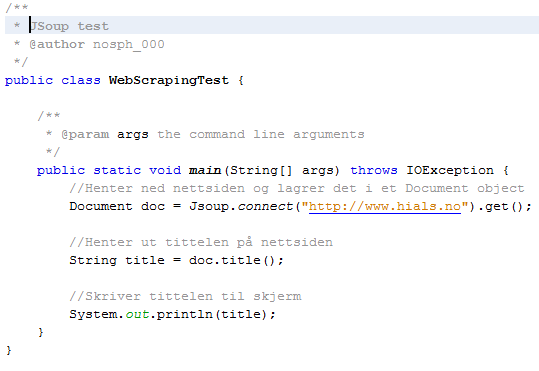
\includegraphics[width=14cm]{jsoup.png}
  \caption{Jasdasdsadsad}
\end{figure}

\subsubsection{RibbonMenu}

Ribbonmenu er et bibliotek for Android som brukes til å presentere data i en meny som kan “skli” inn fra siden av skjermen. Dette biblioteket etterligner den samme funksjonen som man finner i menyen på mobilapplikasjonene FaceBook og Google+. Fordelen med å bruke denne typen meny er at man har plass til mye informasjon og store ikoner i menyen, uten å bruke mye plass på skjermen når man ikke bruker den. En annen fordel er at den følger Google sine retningslinjer om komformitet innen applikasjonsdesign. Det finnes et standard bibliotek fra Google med mye av den samme funksjonen, men denne var ikke tilgjengelig da utviklingen av applikasjonen startet. \endnote{\url{http://developer.android.com/design/patterns/navigation-drawer.html} - 28.05.2013}Dette biblioteket heter Navigation Drawer.

\section{Programverktøy}

Denne delen av rapporten detaljerer de forskjellige programverktøyene som ble benyttet under utviklingen av prosjektet.

\subsubsection{NetBeans}

NetBeans er et integrert utviklings miljø(Integrated Development Environment) som brukes til å utvikle datasystemer. Netbeans er i stand til å ta seg av alle trinnene av utviklingen, som sjekk av syntaks, kompilering av kode og feilsøking av kode. I tillegg finnes det mange moduler som kan legges til som utvider funksjonaliteten. Netbeans blir hovedsakelig brukt til utvikling av Java, HTML5, PHP og C/C++, men kan brukes til andre språk også, avhengig av hvilke moduler som er installert. \endnote{\url{http://en.wikipedia.org/wiki/NetBeans} - 29.05.2013}

\subsubsection{GlassFish}

Glassfish er en applikasjonsserver for Java Enterprise Edition webapplikasjoner. Glassfish støtter alle Java Enterprise Edition teknologiene som: JavaServer Faces, JavaServer Pages, Enterprise JavaBeans osv. \endnote{\url{http://en.wikipedia.org/wiki/GlassFish}}

\subsubsection{Git}

Git er et distribuert versjonskontrollsystem for programvareutvikling. \endnote{Git Pro, Forfatter: Scott Chacon , Forlag Apress, ISBN-10 1430218339} Git er ideelt til teambasert programmering da det gjør det mye letter å slå sammen filer og endringer gjort av de individuelle teammedlemmene. Et Git prosjekt består av en mappe der alle endringer blir lagret som revisisjoner (commits). Disse revisjonene blir organisert med full historikk slik at bidragsyterene i prosjektet kan se hvem som har gjort hvilke endringer og "rulle tilbake" endringer som ikke er ønskelige. \endnote{\url{http://en.wikipedia.org/wiki/Git_(software)} - 28.05.13} \endnote{\url{https://netbeans.org/features/index.html} - 30.05.2013}

\subsection{Android}

\subsubsection{Beskrivelse}

Android er et operativsystem hovedsaklig beregnet for mobile og små enheter med berøringsskjerm. Det er verdens mest brukte operativsystem på mobile enheter, og er stadig i vekst. \endnote{\url{http://developer.android.com/about/index.html} - 30.04.2013 13:29} Mye av populariteten til Android kommer av at det er tilgjengelig på et bredt utvalg av maskinvare og i alle prisklasser. \endnote{\url{http://www.android.com/about/} - 28.05.2013} For produsentene sin del er Android populært da det er hovedsakelig åpen kildekode \endnote{\url{http://developer.android.com/about/index.html} - 28.05.2013} og dermed billig å levere med sine enheter. Mange av produsentene modifiserer også operativsystemet noe for å gjøre det til sitt eget, men dette er hovedsakelig grafiske forandringer.\newline
Android er populært hos utviklerene da det er et mer åpent operativsystem. Dette gjør at det er lettere å utvikle applikasjoner, og at de kan bli bedre integrert i den totale brukeropplevelsen ved telefonen. \endnote{\url{http://www.passion4teq.com/articles/ios-android-development-comparison-2/} - 28.05.2013}

\subsubsection{Teknisk}

Android er basert på en åpen kildekode linux kjerne og er skrevet i C, C++ og Java. Alle applikasjoner som blir levert til Android er skrevet i Java og og bruker XML. Dette blir kompilert om for bruk i Android sin Dalvik virtual Machine(som er Android sin version av Java Virtual Machine).\newline
\newline
Android applikasjoner er bygd opp av to hovedkomponenter. Disse er såkalte "aktiviteter" \endnote{\url{http://developer.android.com/guide/components/activities.html} - 28.05.2013} og "tjenester"(service) \endnote{\url{http://developer.android.com/guide/components/services.html} - 28.03.2013}. En aktivitet er den delen som vises på skjermen, og kjører kun så lenge den blir vist på skjermen. En typisk applikasjon består av flere aktiviteter hvor man kan navigere mellom disse. 
I tillegg kan hver aktivitet ha flere "fragmenter". Et fragment kan inneholde logikk og et grafisk grensesnitt, men må alltid være en del av en aktivitet. Flere fragmenter kan kombineres for å lage en samling med forskjellige brukergrensesnitt i samme skjermbilde. \endnote{\url{http://developer.android.com/guide/components/fragments.html}} \newline
En tjeneste er en bakgrunnsprosess som kan kjøre selv om man bytter mellom aktiviteter. Tjenestene blir ofte brukt til ting som IO og mellomlagring av globale variabler.

\newpage

\end{document}